\documentclass[titlepage]{article}
\usepackage{babel}
\usepackage{amsmath}
\usepackage{amssymb}
\usepackage{amsthm}
\usepackage{multicol} %spalten in seite
\usepackage{graphicx} %bilder einfügen
\usepackage[normalem]{ulem} %durchstreichen
\usepackage{tabto} %tabulator mit \tab
\usepackage{hyperref}
\usepackage{tikz}
\usetikzlibrary{shapes.geometric}
\usepackage{wasysym}
\usepackage{bbm}
\usepackage{bbold}
\usepackage{xcolor}
\usepackage[T1]{fontenc}

\usepackage{mathrsfs}  
\usepackage[utf8]{inputenc}
\usepackage{listings} %quellcode
\pagestyle{plain}
\pagenumbering{arabic}
\renewcommand{\arraystretch}{1.3} %vertikaler abstand von tabellen
\newcommand{\n}{\newline}
\usepackage[left=20mm, right=15mm, top=10mm, bottom=7mm, paper=a4paper]{geometry}
\renewcommand{\contentsname}{Inhaltsverzeichnis}

\newcommand{\K}{\mathbb{K}}
\newcommand{\C}{\mathbb{C}}
\newcommand{\N}{\mathbb{N}}
\newcommand{\Q}{\mathbb{Q}}
\newcommand{\R}{\mathbb{R}}
\newcommand{\1}{\mathbb{1}}
\newcommand{\0}{\mathbb{0}}
\newcommand{\Z}{\mathbb{Z}}
\newcommand{\T}{\mathbb{T}}

\newcommand{\vecD}[3]{\left(\begin{smallmatrix}#1\\#2\\#3\end{smallmatrix}\right)}
\newcommand{\matrixZ}[4]{\begin{pmatrix}#1&#2\\#3&#4\end{pmatrix}}
\newcommand{\detZ}[4]{\begin{vmatrix}#1&#2\\#3&#4\end{vmatrix}}
\newcommand{\smallMatrixZ}[4]{\left(\begin{smallmatrix}#1&#2\\#3&#4\end{smallmatrix}\right)}
\newcommand{\smallDetZ}[4]{\left|\begin{smallmatrix}#1&#2\\#3&#4\end{smallmatrix}\right|}
\newcommand{\vecZ}[2]{\left(\begin{smallmatrix}#1\\#2\end{smallmatrix}\right)}
\newcommand{\detD}[9]{\begin{vmatrix}#1&#2&#3\\#4&#5&#6\\#7&#8&#9\end{vmatrix}}

\newcommand{\sarrusD}[9]{(#1)\cdot(#5)\cdot(#9)+(#4)\cdot(#8)\cdot(#3)+(#7)\cdot(#2)\cdot(#6)-(#7)\cdot(#5)\cdot(#3)-(#1)\cdot(#8)\cdot(#6)-(#4)\cdot(#2)\cdot(#9)}

\begin{document}
	
	\begin{center}
		
\begin{tikzpicture}
			\draw (0,0) node[draw, rectangle]{\textsc{Wintersemester 2020/21}};
		\end{tikzpicture}
		\hrulefill\\
		\begin{center}
			\LARGE\textsc{Lineare Algebra - Übung 10} \normalsize\\
		\end{center}
		\hrulefill
		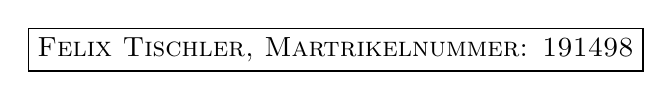
\begin{tikzpicture}
			\draw (0,0) node[draw, rectangle]{\textsc{Felix Tischler, Martrikelnummer: 191498}};
		\end{tikzpicture}
		\date{\today}
	\end{center}
	
	\section*{Hausaufgaben (Abgabe bis 25.01.2021, 14:00 Uhr)}
		\paragraph{Hausaufgabe 10.1:} (4 P.) Sei $\K$ ein Körper und $n\in\N^*.$ Zeigen Sie, dass für alle $x_1,\dots,x_n\in\K$ gilt gilt:
		\begin{align*}
			det\left(\begin{smallmatrix}
				1&1&\dots&1\\
				x_1&x_2&\dots&x_n\\
				x^2_1&x^2_2&\dots&x^2_n\\
				x^3_1&x^3_2&\dots&x^3_n\\
				\vdots&\vdots&\ddots&\vdots\\
				x_1^{n-1}&x_2^{n-1}&\dots&x_n^{n-1}
			\end{smallmatrix}\right)
			=\prod_{1\le i\le j\le n}^{}(x_j-x_i).
		\end{align*}
		\subsection*{$Induktionsanfang$} falls: $n=1$\\
		\scalebox{1.2}{\parbox{.5\linewidth}{%
				\begin{align*}
					|1|=\prod1\checked
				\end{align*}
		}} \\
		falls: $n=2$\\
		\scalebox{1.2}{\parbox{.5\linewidth}{%
				\begin{align*}
					\detZ{1}{1}{x_1}{x_2}\overset{Sarrus}{=}x_2-x_1\checked
				\end{align*}
		}}
		\subsection*{$Induktionsvoraussetzung$ $IV$}
		mit: $n=k\in\N^*$\\
		\scalebox{1.2}{\parbox{.5\linewidth}{%
				\begin{align*}
					\left|\begin{smallmatrix}
						1&1&\dots&1\\
						x_1&x_2&\dots&x_k\\
						x^2_1&x^2_2&\dots&x^2_k\\
						\vdots&\vdots&\ddots&\vdots\\
						x_1^{k-1}&x_2^{k-1}&\dots&x_k^{k-1}
					\end{smallmatrix}\right|=\prod_{1\le i\le j\le k}^{}(x_j-x_i)
				\end{align*}
		}}
		\subsection*{$Induktionsbehauptung$}
		mit: $n=k+1$\\
		\scalebox{1.2}{\parbox{.5\linewidth}{%
				\begin{align*}
					\left|\begin{smallmatrix}
						1&1&\dots&1\\
						x_1&x_2&\dots&x_{k+1}\\
						x^2_1&x^2_2&\dots&x^2_{k+1}\\
						\vdots&\vdots&\ddots&\vdots\\
						x_1^{k}&x_2^{k}&\dots&x_{k+1}^{k}
					\end{smallmatrix}\right|=\prod_{1\le i\le j\le k+1}^{}(x_j-x_i)
				\end{align*}
		}}
		\subsection*{$Induktionsbeweis$}
		\scalebox{1.2}{\parbox{.5\linewidth}{%
				\begin{align*}
					\left|\begin{smallmatrix}
						1&1&\dots&1\\
						x_1&x_2&\dots&x_{k+1}\\
						x^2_1&x^2_2&\dots&x^2_{k+1}\\
						\vdots&\vdots&\ddots&\vdots\\
						x_1^{k}&x_2^{k}&\dots&x_{k+1}^{k}
					\end{smallmatrix}\right|
					\overset{(1)}{\rightsquigarrow}
					\left|\begin{smallmatrix}
						1&0&\dots&0\\
						x_1&x_2-x_1&\dots&x_{k+1}-x_1\\
						x^2_1&x^2_2-x^2_1&\dots&x^2_{k+1}-x^2_1\\
						\vdots&\vdots&\ddots&\vdots\\
						x_1^{k}&x_2^{k}-x_1^{k}&\dots&x_{k+1}^{k}-x_1^{k}
					\end{smallmatrix}\right|
					\overset{Laplace}{=}1\cdot
					\left|\begin{smallmatrix}
						x_2-x_1&x_3-x_1&\dots&x_{k+1}-x_1\\
						x^2_2-x^2_1&x_3^2-x_1^2&\dots&x^2_{k+1}-x^2_1\\
						\vdots&\ddots&\vdots\\
						x_2^{k}-x_1^{k}&x_3^k-x_1&\dots&x_{k+1}^{k}-x_1^{k}
					\end{smallmatrix}\right|
					\overset{(2)}{\rightsquigarrow}
				\end{align*}
				\begin{align*}
					\prod_{i=2\le k}(x_i-x_1)\cdot
					\left|\begin{smallmatrix}
						1&1&\dots&1\\
						x_2+x_1&x_3+x_1&\dots&x_{k+1}+x_1\\
						\vdots&\ddots&\vdots\\
						\sum\limits_{i=0}^{k-1}(x_{2}^{k-1-i}\cdot x_1^i)&\dots&&\sum\limits_{i=0}^{k-1}(x_{k+1}^{k-1-i}\cdot x_1^i)
					\end{smallmatrix}\right|
					\overset{(3)}{\rightsquigarrow}
					\prod_{i=2\le k}(x_i-x_1)\cdot
					\left|\begin{smallmatrix}
						1&1&\dots&1\\
						x_2&x_3&\dots&x_{k+1}\\
						x^2_2&x_3^2&\dots&x^2_{k+1}\\
						\vdots&\ddots&\vdots\\
						x_2^{k-1}&x_3^{k-1}&\dots&x_{k+1}^{k-1}
					\end{smallmatrix}\right|
				\end{align*}
		}}\newpage
		\scalebox{1.2}{\parbox{.5\linewidth}{%
			\begin{align*}
				\overset{IV}{=}
				\prod_{i=2\le k}(x_i-x_1)\cdot
				\prod_{2\le i\le j\le k+1}(x_i-x_j)
				=\prod_{1\le i\le j\le k+1}^{}(x_j-x_i)\qed
			\end{align*}
		}}
		\begin{enumerate}
			\item Jede Spalte außer der ersten minus die erste.
			\item Aus jeder $i-$ten Spalte $(x_i-x_1)$ heraus skaliert.
			\item Jede Zeile minus $x_1-$fachen der vorherigen Zeile (da die erste Zeile immer 1 ist, kann dieser Schritt erfolgen).
		\end{enumerate}
		
		\paragraph{Hausaufgabe 10.2:} \textit{Einige kleine Beweise}
			Sei $\K$ ein Körper, $n\in N^*$ und $A\in M_n(\K).$ Zeigen Sie:
			\begin{enumerate}
				\item[]
				\begin{enumerate}
					\item (1 P.) $\forall B\in M_n(\K):$ Spur($A\cdot B$)=Spur($B\cdot A$).
					\item (2 P.) Wenn $S\in GL_n(\K)$ und $B:=S^{-1}AS,$ dann $\chi_B(X)=\chi_A(X)$.
					\item (1 P.) Sei $V$ ein endlich dimensionaler $\K-$Vektorraum mit Basen $B_1,B_2$ und $\varphi:V\rightarrow V$ ein Endomorphismus. Sei $A_1:={}^{B_1}_{B_1}\varphi$ und $A_2:={}^{B_2}_{B_2}.$ Zeigen Sie $\chi_{A_1}(X)=\chi_{A_2}(X).$ 
				\end{enumerate}
			\end{enumerate}
			(a)
			\begin{align*}
				spur(A\cdot B)=\sum^n_{i=1}(A\cdot B)_{i,i}=\sum^n_{i=1}(\sum^n_{j=1}A_{i,j}B_{j,i})\overset{komm.}{=}\sum^n_{i=1}(\sum^n_{j=1}B_{j,i}A_{i,j})=\sum^n_{i=1}(B\cdot A)_{i,i}=spur(B\cdot A)\qed
			\end{align*}
			(b)
			\begin{align*}
				\chi_B(X)=&det(X\1_n-S^{-1}AS)=det(S^{-1}X\1S-S^{-1}AS)=det(S^{-1}(X\1-A)S)\\
				\overset{Produktregel}{=}&det(S^{-1})\cdot det(X\1-A)\cdot det(S)\overset{Lemma\,5.5}{=}=\underbrace{det(S)^{-1}\cdot det(X\1-A)\cdot det(S)}_{det(S)^{-1}\cdot det(S)=1}\\
				=&det(X\1-A)=\chi_A(X)\qed
			\end{align*}
			(c) In diesem Fall gilt $\underbrace{^{B_1}_{B_1}\varphi={}^{B_1}_{B_2}\T\cdot{}^{B_2}_{B_2}\varphi\cdot{}^{B_2}_{B_1}\T}_*$ nach Beobachtung 4.6 im Skript.
			\begin{align*}
				\chi_{A_1}(X)=det(X\1-{}^{B_1}_{B_1}\varphi)\overset{*}{=}det(X\1-\underbrace{{}^{B_1}_{B_2}\T\cdot{}^{B_2}_{B_2}\varphi\cdot{}^{B_2}_{B_1}\T}_{\underbrace{{}^{B_1}_{B_2}\T\cdot{}^{B_2}_{B_1}\T=1}_{\textsc{Korollar 4.21}}})=det(X\1-{}^{B_2}_{B_2}\varphi)
			\end{align*}
		\paragraph{Hausaufgabe 10.3:} \textit{Berechnung von Eigenräumen}\\
			Sei $A:=\left(\begin{smallmatrix}
				1&-1&-2\\
				-1&1&-2\\
				-2&-2&-2
			\end{smallmatrix}\right)\in M_3(\Q).$\\
			(4 P.) Berechnen Sie die Eigenwerte von $A$ sowie jeweils Basen der zugehören Eigenräume. \textbf{Hinweise:} Die Eigenwerte sind kleine ganze Zahlen; einer der Eigenräumen ist zweidimensional.
			\begin{align*}
				\lambda\textit{ ist Eigenwert von A}\Leftrightarrow\chi_A(\lambda)\Leftrightarrow\underbrace{ det(X\1-A)=0}_*
			\end{align*}
			\begin{align*}
				(*)\Leftrightarrow\detD{X-1}{1}{2}{1}{X-1}{2}{2}{2}{X+2}\overset{!}{=}0
			\end{align*}
			\begin{align*}
				&\scalebox{0.8}{$\overset{Sarrus}{=}\sarrusD{X-1}{1}{2}{1}{X-1}{2}{2}{2}{X+2}\overset{!}{=}0$}\\
				&\Leftrightarrow(X-1)^2\cdot(X+2)+4+4-4(X-1)-4(X-1)-(X+2)\overset{!}{=}0\\
				&\Leftrightarrow(X^2-2X+1)(X+2)+8-4x+4-4x+4-x-2\overset{!}{=}0\\
				&\Leftrightarrow X^3-12X+16=(X-2)^2(X+4)\overset{!}{=}0\Rightarrow X_{1,2}=2,X_3=-4\Rightarrow\textit{ $A$ hat Eigenwerte $\lambda_{1,2}=2,\lambda_3=-4$}\qed
			\end{align*}
			Eigenvektoren:\\\\
			\indent
			\textit{Für $\lambda_{1,2}=2$:}
			\begin{align*}
				E_{\lambda_{1,2}}(A)&=
				\begin{pmatrix}
					1&1&2&0\\
					1&1&2&0\\
					2&2&4&0
				\end{pmatrix}
				\xrightarrow[]{II=I}
				\begin{pmatrix}
					1&1&2&0\\
					2&2&4&0
				\end{pmatrix}
				\xrightarrow[]{II-2\cdot I}
				\begin{pmatrix}
					1&1&2&0\\
					0&0&0&0\\
				\end{pmatrix}\\
			\end{align*}
			\indent
			D.h. $E_{\lambda_{1,2}}(A)=Span(\vecD{-1}{1}{0},\vecD{-2}{0}{1})$\qed\\\\
		
			\textit{Für $\lambda_3=-4$}
			\begin{align*}
				E_{\lambda_3}(A)=
				\begin{pmatrix}
					-5&1&2&0\\
					1&-5&2&0\\
					2&2&-2&0
				\end{pmatrix}
				\xrightarrow[]{I\leftrightarrows II}
				\begin{pmatrix}
					1&-5&2&0\\
					-5&1&2&0\\
					2&2&-2&0
				\end{pmatrix}
				\xrightarrow[III-2\cdot I]{II+5\cdot I}
				\begin{pmatrix}
					1&-5&2&0\\
					0&-24&12&0\\
					0&12&-6&0
				\end{pmatrix}
			\end{align*}
			\begin{align*}
				\xrightarrow[]{II\leftrightarrows III}
				\begin{pmatrix}
					1&-5&2&0\\
					0&12&-6&0\\
					0&-24&12&0
				\end{pmatrix}
				\xrightarrow[II\cdot12^{-1}]{III+2\cdot II}
				\begin{pmatrix}
					1&-5&2&0\\
					0&1&-1/2&0\\
					0&0&0&0
				\end{pmatrix}
			\end{align*}
			\indent
			D.h. $E_{\lambda_3}(A)=Span(\vecD{1}{1}{2})$\qed
		
\end{document}
